\documentclass[]{article}
\usepackage{mathtools}
\usepackage[pdftex]{graphicx}	
\usepackage{amsmath,amsfonts,amsthm}	
\usepackage{tikz}
\usepackage{listings}
\usepackage{slashbox}
\usetikzlibrary{chains, positioning}
\newtheorem{theorem}{Theorem}[section]
\newtheorem{lemma}[theorem]{Lemma}
\newtheorem{proposition}[theorem]{Proposition}
\newtheorem{corollary}[theorem]{Corollary}
\usepackage{sidecap}
\usepackage{polski}
\usepackage[utf8]{inputenc}
\usepackage[T1]{fontenc}
\theoremstyle{definition}
\newtheorem{definition}{Definition}[section]
\usepackage{caption} 
\captionsetup[table]{skip=10pt}
\usepackage{subfigure}
\usepackage{sidecap}
\sidecaptionvpos{figure}{t}

\lstset{
	language=Python, %% Troque para PHP, C, Java, etc... bash é o padrão
	basicstyle=\ttfamily\small,
	numberstyle=\footnotesize,
	%numbers=left,
	%backgroundcolor=\color{gray!10},
	frame=single,
	tabsize=2,
	rulecolor=\color{black!30},
	title=\lstname,
	escapeinside={\%*}{*)},
	breaklines=true,
	breakatwhitespace=true,
	framextopmargin=2pt,
	framexbottommargin=2pt,
	inputencoding=utf8,
	extendedchars=true,
	literate={ą}{{\k a}}1 {ę}{{\k e}}1,} %{ś}{{\'s}}1,

\usetikzlibrary{calc,arrows}

%opening
%\title{Keras}
\author{Rafa\l \vspace{1cm} Skrzypiec}
%\date{}
\begin{document}
%\maketitle

%\section{Keras}
{\large Rafał Skrzypiec - Analiza}\\
Kilka niezależnych paragrafów

\section{Walidacja krzyżowa}

Algorytm wykorzystywany podczas nauki modelu ma za zadnianie znalezienie takich parametrów, które sprawiają, że model odwzorowuje dane wykorzystane do nauki w sposób jak najlepszy z możliwych. Jeśli do walidacji modelu wykorzystamy inną, niezależną próbkę danych pochodzącą z tego samego zbioru co podzbiór uczący, zazwyczaj okaże się, że model nie działa aż tak dobrze jak przy użyciu zbioru uczącego. Rozmiar tej różnicy zwiększa się, szczególnie wtedy gdy wielkość zbioru treningowego jest niewielka, lub gdy liczba parametrów modelu jest bardzo duża.
Walidacja krzyżowa to metoda statystyczna, która ma za zadanie zminimalizować tę różnicę przez co pomaga ocenić i zwiększyć trafność przewidywań modelu predykcyjnego. 


W najprostszym przykładzie walidacji krzyżowej zbiór danych dzieli się na dwa podzbiory: uczący i walidacyjny. Podczas gdy zbiór uczący służy do nauki modelu, zbiór walidacyjny wykorzystuje się aby mierzyć błąd modelu na nieznanym zbiorze danych. 
		
W algorytmie $k$-krotnej walidacji krzyżowej zbiór danych jest losowo dzielony na $k$ równych wielkością podzbiorów. Jeden z $k$ podzbiorów jest przeznaczany na zbiór walidacyjny, pozostałe $k-1$ podzbiorów służą jako dane teningowe. Powyżej opisana procedura jest powtarzana $k$ razy, a każdy $k$ podzbiorów dokładnie raz zostaje wykorzystany jako zbiór testowy. Następnie $k$ wyników modelu jest uśrednianych dając w rezultacie jeden wynik. \figurename{} \ref{fig:cross-val} przedstawia sposób działania $10$-krotnej walidacji krzyżowej.

	\begin{figure}[htp!]
		\centering
		\includegraphics[width=1\textwidth]{cross_val.png}
		\caption{Na podstawie [Python Machine Learning
			Book by Sebastian Raschka]}
		\label{fig:cross-val}
	\end{figure}

Cytując [Page 184, An Introduction to Statistical Learning, 2013.], "(...) istnieje pewien kompromis między obciążeniem a wariancją, związany z wyborem parametru $k$ w $k$-krotnej walidacji krzyżowej. Zazwyczaj stosuje się wartości z przedziału od 5 do 10, ponieważ pokazano empirycznie, że w takim wypadku otrzymujemy przewidywania, które nie cierpią nadmiernie ani z powodu dużego obciążenia ani dużej wariancji." Podczas treningu modelu wybrano $k = 6$, wykorzystując fakt, że liczba próbek w zbiorze danych jest całkowicie podzielna przez tę liczbę co zapewnia równy rozmiar wszystkich zbiorów treningowych i walidacyjnych.

\section{Wczesne zatrzymanie}
Algorytmy uczenia maszynowego dopasowują parametry modelu na podstawie danych treningowych o skończonym rozmiarze. Podczas procesu szkolenia model jest oceniany na podstawie tego, jak dobrze przewiduje obserwacje zawarte w tym zbiorze. Jednak celem uczenia maszynowego jest stworzenie modelu, który ma zdolność do przewidywania uprzednio niewidzianych obserwacji. Nadmierne dopasowanie to zjawisko pojawiające się wtedy gdy model za bardzo dopasowuje się do danych w zbiorze uczącym co powoduje zmniejszenie wartości błędu na tym zbiorze lecz równocześnie jest przyczyną wzrostu błędu na zbiorze testowym. Nadmierne dopasowanie modelu to problem, który może się pojawiać gdy model zawiera więcej parametrów niż wymagałaby tego natura modelowanego zjawiska. Sieć neuronowa to struktura skłonna do przeuczania. Podczas gdy obserwowany błąd obliczany w oparciu o dane treningowe spada, w pewnym momencie wartość błędu dla zbioru walidacyjnego zaczyna wzrastać. \figurename{} \ref{fig:loss_curves} przedstawia często zamieszczane w literaturze, wyidealizowane krzywe zmiany wartości funkcji straty w czasie, dla zbiorów treningowego i walidacyjnego. Najlepszy model predykcyjny miałby parametry, które odpowiadają momentowi globalnego minimum dla zbioru walidacyjnego.


\begin{figure}[htp!]
	\centering
	\includegraphics[width=1\textwidth]{early_stopping14_8.png}
	\caption{Wyidealizowane przykłady krzywych przedstawiających zmianę wartości funkcji straty na zbiorach treningowym i walidacyjnym, podczas nauki modelu}
	\label{fig:loss_curves}
\end{figure}

W dziedzinie uczenia maszynowego, metoda wczesnego zatrzymania to forma regularyzacji, która pozwala uniknąć problemu przeuczenia, zatrzymując naukę modelu gdy wartość funkcji straty na zbiorze walidacyjnym zaczyna wzrastać. Rzeczywisty przebieg wartości funkcji straty ma wiele lokalnych minimów, dlatego na podstawie obserwacji krzywych uczenia dokonano wyboru kryteriów zatrzymania nauki modelu. 
 Niech $\Theta_{wa}(t)$ to wartość funkcji straty na zbiorze walidacyjnym po $t$ epokach, $\Theta_{min}(t)$ to dotychczasowe minimum funkcji straty na zbiorze walidacyjnym po $t$ epokach, definiowane jako:
 $$
 \Theta_{min}(t) \equiv \min_{t' < t} \Theta_{wa}(t')
 $$
 
 Niech $\Theta_{sr}(t)$ będzię średnią wartością funkcji straty dla zbioru walidacyjnego z ostatnich 10 epok.
 
 $$
 \Theta_{sr}(t) \equiv \frac{1}{10} \sum_{i=0}^{10} \Theta_{wa}(t-i)
 $$
 
 Oraz zdefiniujmy pomocniczy parametr $GL(t)$
 
 
 $$
 GL(t) \equiv \frac{\Theta_{sr}(t)}{\Theta_{min}} - 1
 $$
 
 
 Podczas nauki przedstawioneg modelu, do wczesnego zatrzymania wystarczyło spełnienie jednego z dwóch obowiązujących warunków:

\begin{itemize}
\item $\Theta_{min}(t) = \Theta_{min}(t+ 200)$ dla wszystkich $t \in [t,t+200]$, brak zmniejszenia minimalnej wartości funkcji straty dla zbioru walidacyjnego przez 200 epok 
\item $ GL(t)  > 2$, względny wzrost średniej wartości funkcji straty przez ostatnie 10 epok względem osiągniętego minimum jest większy niż $200\%$
\end{itemize}

Po skończeniu nauki, wybierany jest model, który ma najmniejszą wartość funkcji straty na zbiorze testowym.

\section{Ilość neuronów}

Architektura sieci neuronowej, tzn. ilość warstw ukrytych oraz ilość neuronów w warstwach ukrytych jest zdeterminowana przez wymiar danych wejściowych, rodzaj rozwiązywanego problemu (klasyfikacja czy regresja) oraz relację między zmiennymi objaśniającymi i zmienną objaśnianą.

Uogólniony model liniowy przydatny w szerokim zakresie zastosowań, nie potrzebuję żadnej warstwy ukrytej. Bywa szczególnie przydatny gdy zbiór zawiera mało danych lub są one obarczone dużą niedokładnością. Nawet w przypadku gdy relacja między zmiennymi jest lekko nieliniowa, użycie prostego modelu liniowego może skutkować lepszym uogólnieniem problemu niż skomplikowany model będący wrażliwy na każdy szum znajdujący się w danych. Zgodnie z uniwersalnym twierdzeniem aproksymacyjnym jedna warstwa ukryta z wystarczająco dużą liczbą neuronów wystarcza aby z dowolną dokładnością dowolną ciągłą funkcję [cybenko]. Jeśli zmienna objaśniająca jest jednowymiarowa, wydaje się, że nie odniesiemy żadnej korzyści z skonstruowania sieci neuronowej o więcej niż jednej warstwie ukrytej. Sprawy komplikują się jednak gdy zmienna wejściowa jest dwu lub więcej wymiarowa. Dwuwarstowa sieć neuronowa zachowuje właściwości jednowarstwowej sieci neuronowej oraz osiąga zdolność nauki każdego problemu klasyfikacyjnego [1995 Bishop 123], ponadto wielowarstwowa sieć neuronowa z dwoma warstwami może skutkować dokładniejszymi wynikami wykorzystując mniejszą ilość parametrów niż jednowarstwowa sieć [Chester (1990)]. Na tej podstawie, do rozwiązania problemu regresji gdzie wejściem jest para liczb $(\varepsilon, Q^2)$ postanowiłem wybrać sieć neuronowa z dwoma warstwami ukrytymi. 


\begin{table}
	\centering
	
	\caption{Liczba parametrów sieci neuonowej z dwoma warstwami ukrytymi w zależności od liczby neuronów w warstwach}\label{tab:parameters_table} 
	
	
	\begin{tabular}{c|p{1cm}|p{1cm}|p{1cm}|p{1cm}}
		\backslashbox{I warstwa}{II warstwa} & 2 & 3 & 4 & 5\\\hline\hline
		2 & 14 & 18 & 22 & 26 \\ \hline
		3 & 19 & 24 & 29 & 34 \\ \hline
		4 & 24 & 30 & 36 & 42 \\ \hline
		5 & 29 & 36 & 43 & 50 \\ \hline
	\end{tabular}
\end{table}

Aby znaleźć odpowiednią liczbę neuronów w dwóch warstwach ukrytych, stworzyłem siatkę [2, 3, 4, 5] $\times$ [2, 3, 4, 5] neuronów i sprawdziłem, która konfiguracja daje najmniejszy błąd zbioru walidacyjnego. Dane zostały podzielone na zbiór treningowy i testowy w stosunku 2:1. Dla każdej konfiguracji wytrenowano 50 sieci i sprawdzono jak wygląda statystyka błędu. \tablename{} \ref{tab:parameters_table} zawiera porównanie liczby parametrów sieci neuronowej w zależności od liczby neuronów w warstwach ukrytych. Do eksperymentów wybrano konfiguracje charakteryzujące się rozsądną w porównaniu do rozmiaru danych wejsciowych liczbą parametrów. \figurename{} \ref{fig:neurony} przedstawia rozkłady minimalnej wartości funkcji straty uzyskanej na danych walidacyjnych uzyskanej z 50 treningów sieci dla każdej konfiguracji ilości neuronów. Wykres pudełkowy to forma graficznej prezentacji rozkładu, która pozwala w łatwy sposób ukazać położenie, rozproszenie oraz kształt empirycznego rozkładu badanej cechy statystycznej. Konfiguracja 3 $\times$ 5 charakteryzuje się najniższą medianą wartości funkcji straty oraz małą liczbą wartości odstających. Ta obserwacja pozwoliła zdecydować, że liczby neuronów będą wynosiły 3 i 5 w odpowiednio pierwszej i drugiej warstwie ukrytej, co za tym idzie sieć będzie miała 36 parametrów.



%opisać liczbę parametrów + poniższy obrazek

\begin{figure}[htp!]
	\centering
	\includegraphics[width=1\textwidth]{neuronyy14_8.png}
	\caption{Wykresy pudełkowe przedstawiające rozkład wartości funkcji straty w zależności od ilości neuronów w pierwszej i drugiej warstwie ukrytej}
	\label{fig:neurony}
\end{figure}


\begin{SCfigure}
\centering
\resizebox{7.cm}{!}{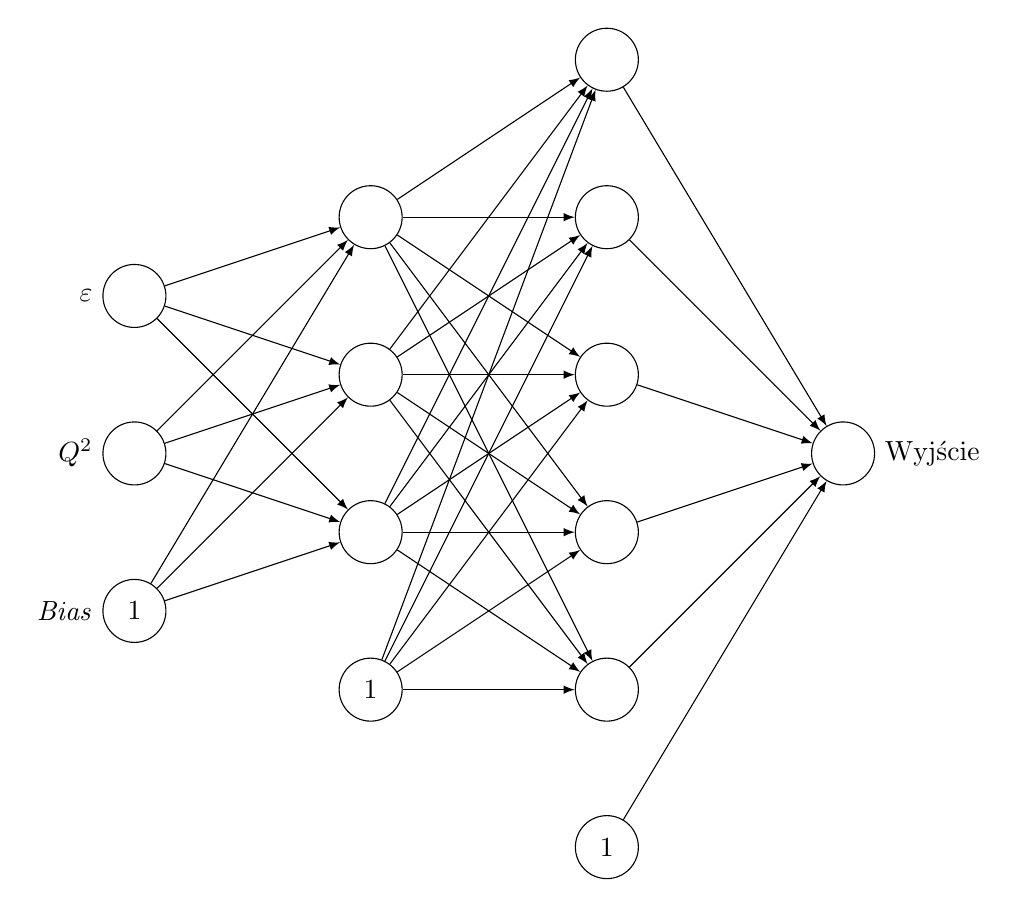
\begin{tikzpicture}
	[   cnode/.style={draw=black,draw=black,fill=#1,minimum width=8mm,circle},
	]
	\tikzset{normal arrow/.style={draw,-latex}}
	\node[cnode=white,label=0:Wyjście] (s) at (9,-7) {};
	
	\node[cnode=white,label=180:\textit{Bias}] (x-3) at (0,-9) {1};

	
	\node[cnode=white,label=180:] (p-4) at (3,-10) {$1$};
	
	\node[cnode=white,label=180:] (z-6) at (6,-12) {$1$};	
	
	
	\node[cnode=white,label=180:$\varepsilon$] (x-1) at (0,-5) {};
	\node[cnode=white,label=180:$Q^2$] (x-2) at (0,-7) {};

	\node[cnode=white,label=180:] (p-1) at (3,-4) {};
	\node[cnode=white,label=180:] (p-2) at (3,-6) {};
	\node[cnode=white,label=180:] (p-3) at (3,-8) {};
	
	\node[cnode=white,label=180:] (z-1) at (6,-2) {};
	\node[cnode=white,label=180:] (z-2) at (6,-4) {};
	\node[cnode=white,label=180:] (z-3) at (6,-6) {};
	\node[cnode=white,label=180:] (z-4) at (6,-8) {};
	\node[cnode=white,label=180:] (z-5) at (6,-10) {};
	


	\foreach \x in {1,...,6}
	{
		\path[normal arrow] (z-\x) -- node[above,sloped,pos=0.4] {} (s);
	}
	
	
	\foreach \x in {1,...,3}
	{   
		\foreach \y in {1,...,3}
		{   

			\path[normal arrow] (x-\x) -- (p-\y); 				
		}
	}

	\foreach \x in {1,...,4}
	{   
	\foreach \y in {1,...,5}
	{   
		
		\path[normal arrow] (p-\x) -- (z-\y); 
	}
		
	\ifnum \x=5
	\path[normal arrow] (z-\x) -- node[above,sloped,pos=0.4] {} (s);
	\else
	
	\fi
	}
\end{tikzpicture}}
\caption{Schemat zastosowanej sieci neuronowej, która składa się z: i) warstwy wejściowej z dwoma neuronami, ii) dwóch warstw ukrytych z odpowiednio trzema i pięcioma neuronami, iii) warstwy wyjściowej z jednym neuronem. Linie zakończone strzałką oznaczają wagę odpowiadającą każdej z par neuronów} \label{tab:scheme} 	
\end{SCfigure}

\section{Algorytm uczący}
 

Bardzo istotnym elementem tworzonego modelu jest wybór algorytmu poszukującego minimum funkcji straty oznaczonej na potrzeby tego paragrafu jako $J(\theta)$. Na podstawie jego wyników aktualizowane będą parametry tworzonej sieci neuronowej. Bardzo pomocną koncepcją pozwalającą zrozumieć istotę trudności problemu jest powierzchnia błędu "\textit{Każda z N wag i wartości progowych sieci (tzn. wszystkie wolne parametry modelu) traktowana jest jako jeden z wymiarów przestrzeni. W ten sposób każdy stan sieci, wyznaczony przez aktualne wartości jej N parametrów może być traktowany jako punkt na N-wymiarowej hiperpłaszczyźnie. N+1 wymiarem (zaznaczanym jako wysokość ponad wspomnianą wyżej hiperpowierzchnią) jest błąd, jaki popełnia sieć. Dla każdego możliwego zestawu wag i progów może więc zostać narysowany punkt w przestrzeni N+1 wymiarowej, w taki sposób, że stan sieci wynikający z aktualnego zestawu jej parametrów lokuje ten punkt na wspomnianej wyżej N-wymiarowej hiperpłaszczyźnie zaś wartość błędu, jaki popełnia sieć dla tych właśnie wartości parametrów stanowi wysokość umieszczenia punktu ponad tą płaszczyzną. Gdybyśmy opisaną procedurę powtórzyli dla wszystkich możliwych wartości kombinacji wag i progów sieci, wówczas otrzymalibyśmy "chmurę" punktów rozciągających się ponad wszystkimi punktami N-wymiarowej hiperpłaszczyzny parametrów sieci, tworzącą właśnie rozważaną powierzchnię błędu. Celem uczenia sieci jest znalezienie na tej wielowymiarowej powierzchni punktu o najmniejszej wysokości, czyli ustalenie takiego zestawu wag i progów, który odpowiada najmniejszej wartości błędu.
Przy stosowaniu modeli liniowych z funkcją błędu opartą na sumie kwadratów powierzchnia błędu ma kształt paraboloidy (funkcji kwadratowej), ma więc kształt kielicha o gładkich powierzchniach bocznych i o jednym wyraźnym minimum. Z tego powodu wyznaczenie w tym przypadku wartości minimalnej nie stwarza większych problemów.}"[$https://www.statsoft.pl/textbook/stathome_stat.html?$]

Jeżeli dysponujemy niewielkim zbiorem danych treningowych, do znalezienia optimum funkcji doskonale sprawdzą się metody quasi-Newtonowskie. Ich zaletą jest bardzo szybka zbieżność, niestety obliczenie hesjanu funkcji wielu zmiennych charakteryzuje się dużą złożonością pamięciową $O(n^2)$ i jeszcze większą złożonością obliczeniową $O(n^3)$. Z tego powodu możliwość ich zastosowania ogranicza się do niewielu przypadków. Najbardziej znane algorytmy quasi-Newtonowskie to m.in: \textit{LM-BFGS, Levenberg-Marquardt.} Dysponując dużym zbiorem danych należy wybrać inny algorytm. Po za losowym poszukiwaniem parametrów, najłatwiejszym z nich i bardzo intuicyjnym jest metoda gradientu prostego (\textit{gradient descent}). Parametry $\theta$ aktualizowane są w następujący sposób:


\begin{equation}
\theta^{k+1} = \theta^{k} - \alpha \nabla J(\theta^{k})
\end{equation}


gdzie $\alpha$ to wybrany odpowiednio parametr szybkości uczenia (\textit{learning rate}) odpowiedzialny za stopień zmiany parametrów w kolejnych iteracjach. Jeśli $\theta^0$ znajduje się odpowiednio blisko minimum funkcji, i parametr $\alpha$ jest wystarczcająco niewielki, algorytm osiąga liniową zbieżność [Dennis, J., Schnabel, R.B.: Numerical Methods For Unconstrained Optimization and Nonlinear Equations. Prentice-Hall, Inc., Englewood Cliffs, New Jersey (1983)
]. W ogólności metoda gradientu prostego gwarantuje zbieżność do globalnego minimum w przypadku funkcji błędu o wypukłej powierzchni i do lokalnego minimum dla funkcji błędu o powierzchni nie wypukłej. Algorytm jednak jest bardzo wolny, co jest jego największą słabością. Ze względu na częstość aktualizacji wag, metodę gradientu prostego możemy podzielić na \textit{batch gradient descent} oraz \textit{stochastic gradient descent}. W pierwszym przypadku wagi są dostosowywane po przetworzeniu pełnego zbioru danych, w metodzie stochastycznej zbiór uczący dzielony jest na podzbiory a wagi aktualizowane są po przetworzeniu każdego z podzbiorów. Druga metoda jest szczególnie użyteczna dla dużych zbiorów danych. Spodziewamy się, że dla dobrze przygotowanych danych kierunek podążania wartości wag będzie podobny jeśli policzymy gradient zarówno dla 10\% jak i dla 100\% zbioru treningowego.


Wyobraźmy sobie, że poszukiwanie minimum powierzchni błędu to przemierzanie przestrzeni pełnej dolin, pagórków, wąwozów. W kolejnych iteracjach przeskakujemy między tymi obszarami, w pewnym momencie może się zdarzyć, że gradient zaniknie lub będzie bardzo słaby a nasze poszukiwania zatrzymają się nie osiągając wystarczającego minimum. Idea pędu inspirowana zjawiskami fizycznymi to nadanie gradientowi krótkotrwałej pamięci. Posługując się kolejną analogią, popchnięta w dół piłka nabierając prędkości zwiększa swój pęd. To samo dzieje się z parametrami sieci, wartość pędu wzrasta dla wymiarów, których gradienty wskazują te same kierunki i zmniejsza modyfikacje wartości dla wymiarów, w których gradienty zmieniają kierunki. W rezultacje otrzymujemy szybszą zbieżność i mniejsze oscylacje.

\begin{align} 
v^{k+1} &=  \beta v^{k}+ \nabla J(\theta^{k}) \\[0.4em]
\theta^{k+1} &=  \theta^{k }- \alpha v^{k+1}
\end{align}

Zmiana jest niewielka, gdy $\beta = 0$, otrzymujemy zwykłą metodę gradientu prostego, zazwyczaj jednak ustala się wartość parametru $\beta$, zwanego pędem na około $0.9$. [1986 Nature, Learning representations by back-propagating errors
David E. Rumelhart, Geoffrey E. Hinton \& Ronald J. Williams] 

\begin{figure}[h	]
	\centering
	\includegraphics[width=1\textwidth]{gd_sgd.png}
	\caption{Funkcja  $f(x,y) =(1.5 - x + xy)^2 + (2.25 - x + xy^2)^2 + (2.625 - x + xy^3)^2$, osiąga minimum równe 0, w punkcie $(3,0.5)$ oznaczonym  czarną gwiazdą. Grafika przedstawia porównanie działania metody gradientu prostego oraz jego modyfikacji poprzez dodanie pędu. Przyjmując, że punkt początkowy to $(2,1)$, $\alpha = 0.001$ i $\beta = 0.9$, możemy prześledzić trajektorie algorytmów przez pierwsze 500 iteracji działania.} 
	\label{fig:gd_sgd}
\end{figure}

Porównanie efektywności przedstawionych wyżej algorytmów znajduje się na \figurename{} \ref{fig:gd_sgd}, w zaprezentowanym przykładzie metoda gradientu prostego potrzebuje około 10 razy więcej iteracji od modyfikacji z pędem aby dotrzeć do minimum zaprezentowanej funkcji. Jest to przykład świadczący o tym jak duży wpływ na szybkość działania algorytmu wywiera ta niewieka modyfikacja. 


Wykorzystany podczas treningu modelu algorytm korzysta jednak z jeszcze z jednej modyfikacji. Nie chcielibyśmy aby piłka spuszczona w dół ślepo podążała za zboczem widząc, że za niedługo mocno się ono podniesie. Przyspieszenie Nesterova (\textit{NAG}) jest sposobem na uwzględnienie podczas obliczania gradientu przybliżonej przyszłej pozycji parametrów sieci.	

\begin{align} 
v^{k+1} &=  \beta v^{k}+ \nabla J(\theta^{k} - \beta v^{k}) \\[0.4em]
\theta^{k+1} &=  \theta^{k }- \alpha v^{k+1}
\end{align}
[https://arxiv.org/abs/1609.04747]


Niezywkle istotnym parametrem algorytmu jest $\alpha$, jego niezmienność wraz z postępem iteracji powoduje bardzo niską efektywność algorytmu. Ze względu na metodę zmiany tego parametru, który może być indywidualnie ustalany dla każdej wagi powstało wiele szeroko wykorzystywanych algorytmów. Do najpopularniejszych należą między innymi \textit{Adam, Nadam, Adagrad, Adadelta, AMSGrad, RMSprop}. 

W swoim algorytmie postanowiłem dokonywać zmiany parametru $\alpha$ wraz ze wzrostem iteracji. Ponadto szybkość uczenia zależna jest od wybranego parametru $\lambda$ decydującego o tym z jaką szybkością maleje.

\begin{equation}
\alpha(i) = \alpha_0 \times \frac{1}{1 + \lambda \times i}
\end{equation}

\figurename{} \ref{fig:hyperparameters} przedstawia porównanie przykładowych krzywych zmian wartości funkcji straty w czasie dla różnych wartości $\alpha$ i $\lambda$. Na ich podstawie widać jak duży wpływ wnosi parametr $\alpha$ w proces nauki modelu. Zbyt duża szybkość uczenia powoduje bardzo duże oscylacje krzywej funkcji straty, za mała wartość $\alpha$ bardzo mocno spowalnia proces nauki. Pewien kompromis przynosi wybranie odpowiednio dużej początkowej wartości szybkości uczenia, co przynosi szybkie przejście algorytmu w obszar minimum i następnie zmniejszenie go do wartości potrafiącej efektywnie dalej poszukiwać optimum. Zadowalający przebieg mają krzywe o parametrach $\alpha = 0.005$, $\lambda = 0.001$, które przedstawiają porządany, eksponencjalny kształt o niewielkiej oscylacji. Na podstawie powyższej analizy to właśnie te hiperparametry zostały wykorzystane w modelu, dodatkowo parametr pędu $\beta$ został ustalony na wartość $0.9$


\begin{figure}[htp!]
	\centering
	\includegraphics[width=1\textwidth]{hyperparameter14_16a.png}
	\caption{Porównanie przykładowych krzywych zmiany wartości funkcji straty w czasie dla zbiorów treningowego (kolor pomarańczowy) i walidacyjnego (kolor niebieski) ze względu na parametry $\alpha$ (\textit{learning rate}) oraz $\lambda$ (\textit{decay})}
	\label{fig:hyperparameters}
\end{figure}


\section{Dane wejściowe}

\section{Funkcja straty}

\section{Replikacja danych}
\end{document}


